%
% File acl2014.tex
%
% Contact: giovanni.colavizza@epfl.ch
%%
%% Based on the style files for ACL-2013, which were, in turn,
%% Based on the style files for ACL-2012, which were, in turn,
%% based on the style files for ACL-2011, which were, in turn, 
%% based on the style files for ACL-2010, which were, in turn, 
%% based on the style files for ACL-IJCNLP-2009, which were, in turn,
%% based on the style files for EACL-2009 and IJCNLP-2008...

%% Based on the style files for EACL 2006 by 
%%e.agirre@ehu.es or Sergi.Balari@uab.es
%% and that of ACL 08 by Joakim Nivre and Noah Smith

\documentclass[11pt]{article}
\usepackage{acl2014}
\usepackage{times}
\usepackage{url}
\usepackage{latexsym}
\usepackage{todonotes}
\usepackage[nameinlink]{cleveref}
\usepackage{enumitem}

\setlist[itemize]{leftmargin=*}
\setlength{\belowcaptionskip}{-8pt}
%\setlist{noitemsep}
\setlist{nosep}

%\setlength\titlebox{5cm}

% You can expand the titlebox if you need extra space
% to show all the authors. Please do not make the titlebox
% smaller than 5cm (the original size); we will check this
% in the camera-ready version and ask you to change it back.


\title{Exposing the network beneath Amazon}

\author{Dario Pavllo  \\\And
  Mattia Martinelli  \\\And
Niccolo Sacchi \\}

\date{}

\begin{document}
\maketitle
\begin{abstract}
This project aims to find unobserved patterns and insights that could be useful for Amazon's users. To conduct our research, we devise an algorithm that builds a graph of Amazon products, where similar articles are grouped in an innovative manner. We also define a novel metric to find popular products, and we investigate how it is affected by features in the items, such as their title or rating.
\end{abstract}

\section{Introduction}
Buying from huge e-commerce websites such as \emph{Amazon} has many advantages, but paradoxically, users are often confused by the vast variety of products. Users may have a rough idea about the characteristics of the product they want to buy, and they often undergo the same process of comparing similar products. The goal of this research is to understand why clients tend to choose a product over another, i.e. what are the desirable characteristics of a popular product. Hopefully, we would get some insights that could prove useful for both clients and vendors.
We also aim to identify patterns in the products and their relations. Do brands affect the popularity of product? Can we predict whether a product is preferred to another by looking at its features (e.g. title, ratings). More generally, is it possible to identify the best products among groups of similar ones? 

This report is organised as follows: \Cref{sec:datastruct} briefly explains the dataset structure, \Cref{sec:datapreprocessing} and \Cref{sec:explodatanalysis} describe how we have preprocessed and explored the dataset, \Cref{sec:graphanalysis} reports how we have developed our research, and finally \Cref{sec:conclusion} reports our findings.

\section{Dataset structure}
\label{sec:datastruct}
Our analysis is based on the Amazon reviews/products dataset, which consists of two JSON files: 
\begin{itemize}
	\item \textit{metadata}: contains information related to the products, such as their unique ID (\textit{ASIN}), category, description, \textit{sales rank}, brand, price, and relations with other items. Such relations, which are of fundamental importance for building our graph, indicate how items are bought and visualized together. The size of the file is 9.81 GB (uncompressed).
	\item \textit{reviews}: contains ratings and reviews associated to each product, as well as the helpfulness of each review. The size of the file is approximately 87 GB (uncompressed).
\end{itemize}

\section{Dataset preprocessing}
\label{sec:datapreprocessing}
The dataset, due to its large size, cannot be handled directly using in-memory libraries such as Pandas. Therefore, it has been processed using PySpark, both on the cluster and locally. While it may seem inappropriate, using Spark in local mode is indicated for medium-sized datasets (like the metadata one), as it automatically parallelizes jobs using all cores and spills to disk intermediate results that cannot fit in main memory.

Since the text content of \textit{reviews} was not necessary for our analysis, for each product, we extracted average rating, number of reviews, and their \textit{helpfulness} score. These fields have been then merged with \textit{metadata}.

We noticed that products were distributed over a wide set of categories, therefore, we decided to extract only the most relevant ones. We excluded categories in which purchase decisions tend to depend on people's personal preferences, rather than on an objective evaluation. Examples of such categories are \textit{Music}, \textit{Clothes} and \textit{Books}. As a result, we created a lighter dataset using only five macro-categories in which the market demands for competition: \textit{Electronics}, \textit{Cell Phones \& Accessories}, \textit{Automotive}, \textit{Tools \& Home Improvement}, and \textit{Musical Instruments}. 

\section{Exploratory data analysis}
\label{sec:explodatanalysis}
We investigated what fields can be exploited by analysing missing data, feature distribution and correlations.
\subsection{Missing data}
We observed that the quantity of missing entries significantly varies among the dataset fields. \textit{ASIN} and \textit{category} are always present by definition. In addition, almost all articles have at least one review. On the other hand, \textit{sales rank} and \textit{brand} are missing in about 60\% of cases. The remaining fields are overall present in the dataset, with a missing ratio lower than 30\%.
\subsection{Feature analysis}
\begin{figure}[h]
	\centering{}
	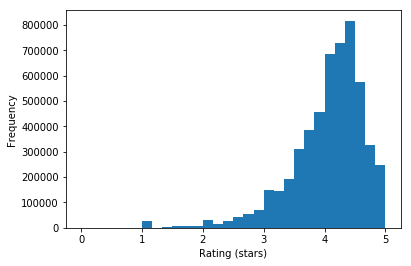
\includegraphics[width=0.47\textwidth]{img/avgReviews.png}
	\caption{Distribution of the \textit{average rating} field.}
	\label{fig:avgdist}
\end{figure}
\Cref{fig:avgdist} shows that ratings tend to be high. This evidence suggests that they may be not a useful metric for evaluating the popularity of a product.
We investigated correlations among \textit{price}, \textit{average rating} and \textit{sales rank}, but their coefficients do not seem to be significant. However, some assumption could be asserted. As the price increases, the ratings tend to have lower variance and higher mean. In other words, expensive products tend to have higher ratings.
As the price increases, the sales rank tends to be lower (i.e. better). Costly products may be regarded as superior by people. 

\section{Graph analysis}
\label{sec:graphanalysis}
In order to analyse patterns and gain insights into the dataset, we devised an algorithm for clustering products with similar characteristics, i.e. \textit{competing products}, by exploiting the graph topology. One of our goals is to compare two products and decide which one is better. Before being able to compare two products, we have to cluster them into comparable products, as it would be meaningless to compare two products with very different characteristics (e.g. a cheap phone with a very expensive one).

The algorithm builds a network of products using the relations between items provided in the dataset. In general terms, such relations have been collected by analysing the behaviour of Amazon's users, i.e. what products they buy or visualise together. We assume that these relations could reflect meaningful patterns, as users tend to compare similar or related products.

\subsection{Graph structure}
The dataset has been transformed into graphs of relations between products, where nodes represent products, and edges represent ``competitions'' between products. To ensure a coherent result and facilitate the computation, the graph includes only products of the same category. Specifically, we built the graph in a way that an edge from product A to product B is added if clients \textbf{buy} B after viewing A (\textit{buy after viewing} relation), but the edge between A and B is removed if A and B are frequently bought together (\textit{bought together} relation). The former means direct competition, i.e. an article has been preferred over another, while the latter means no competition, i.e. the two articles are complementary (e.g. a cellphone and a cover).

In previous experiments, we tried to build the graph by adding edges between products that are viewed together (\textit{also viewed} relation). This relation does not imply that any of the products has been actually bought, and it produces a graph that is too dense to give meaningful results. %Additionally, we believe that the also viewed relation is generated by Amazon's recommender system according to users' preferences, and it does not actually represent a graph relation. \todo{quote needed}

Since we employed an NP-Complete algorithm for our analysis (max-clique extraction), we assumed the graph to be sparse. Indeed, the assumption turned out to be correct.

%\todo[inline]{should cliques and algorithm deserve more space here?}
%\todo{connected components @ dario}
%\todo{cartsimilarities @dario}


\subsection{Graph insights}
By visually inspecting the graph, we identified some common structures.
\begin{itemize}
	\item \textbf{Accumulators:} these are popular products that have many incoming edges.
	\item \textbf{Max-cliques:} groups of products that are totally interconnected. In many cases, these products are also accumulators. Cliques represent products that are in direct competition with each other (and it is not really clear which one ``wins"). Note that these competition relations might even comprehend products of the same brand.
\end{itemize}
\begin{figure}
	\centering{}
	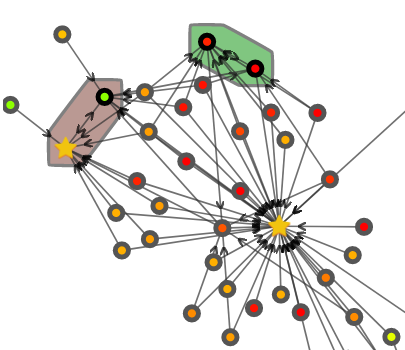
\includegraphics[width=0.45\textwidth]{img/graph.png}
	\caption{Portion of the graph of a category. The stars represent accumulators, whereas the groups represent cliques.}
	\label{fig:graph}
\end{figure}
We wrote algorithms for automatically extracting these patterns and analyzed them to make sure that they were coherent. In particular, for max-cliques, we ran the extraction algorithm on the full graph and verified whether all the products in a clique belong to the same category. This is true in 70\% of cases. Afterwards, we repeated the analysis on strongly connected components and discovered that many products are assigned to the wrong category in a detectable way. We also analyzed some cliques by hand and observed some recurrent patterns: in some cases, they contain the same product in different variations (e.g. color); in other cases, they represent different products from the same manufacturer, and, finally, they can also contain different products from different manufacturers. Since the data appeared to be very consistent, we decided to adopt it without further cleaning.

\subsection{Methodology}
Now that products are represented as nodes of a directed graph, a new feature becomes available: the product \emph{fan-in} (or \emph{in-degree}), which represents the number of incoming edges in a node. Since an incoming edge indicates that a product has been preferred over another one, such a feature could be exploited to measure the popularity of a product. To validate this metric, we investigated correlations between fan-in and other features already included in the dataset, such as sales rank, average rating, and number of reviews.
\begin{figure}
	\centering{}
	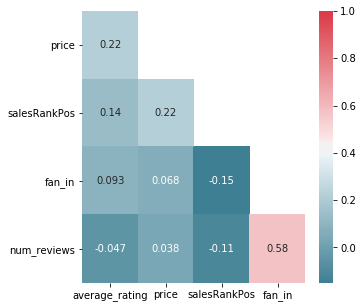
\includegraphics[width=0.45\textwidth]{img/faninCorr.png}
	\caption{Correlations between metrics.}
	\label{fig:faninCorr}
\end{figure}
As shown in \Cref{fig:faninCorr}, the fan-in has a moderate correlation with the number of reviews, and a weak correlation with the sales rank. We also observed a weak correlation between the sales rank and the price, which makes us suppose that people tend to prefer cheaper products. We can conclude that fan-in could be effectively used to measure the \textit{preference} of a product, i.e. how much the product is favoured over the others. In addition, the fan-in shows several advantages over the other features. As mentioned in \Cref{sec:explodatanalysis}, the sales rank is present only in 60\% of the products. Moreover, it has a coarse granularity (i.e. it is computed only on macro-categories), and it continuously evolves over time (which adds noise to the data).

\subsection{Predicting the best products}
We investigated how people decide when they are presented with a choice. To do this, we trained a classifier (analysing both textual and numerical features) to predict the preferred product (i.e. the one with the highest fan-in) within a group of related products. Afterwards, we interpreted its features and observed what words/fields correlate with the best products. Going into more depth, our model compares pairs of products and emits a binary label that corresponds to the index of the ``winner''. In the \textit{learning to rank} context, such approach is known as the \textit{pairwise approach} \cite{Li:11}.
Textual features are extracted from the titles (using a tf-idf vectorizer), as they represent a direct  and easy-to-interpret description of the product. For the actual comparison task, we subtract the feature vectors of the two products to produce the feature vector to supply to the classifier. As for the ground truth, provided that the subtraction is $A - B$, we put the label 0 if the winner is A, and 1 if the winner is B. For each sample, we also provide the opposite sample ($B - A$ with the inverted label), so that the classifier learns the commutative property and the classes are perfectly balanced.
Afterwards, we train a random forest on our data, with a fixed number of estimators (1000) and an optimal tree depth which is determined by grid search and cross-validation. Moreover, we evaluate our model on a small test set (20\% of the data) to determine whether it overfitted or not. The next step is the interpretation, which is done by selecting the most important features learned by the random forest. However, this is not sufficient, as we get only an indication of their magnitude (a positive value), and not whether they affect positively or negatively the result.
To get an idea of their impact, we select the top 1000 features (i.e. words) in terms of importance, and we use them to train a L2-regularized logistic regressor. By analyzing the weights learned by the latter, we can observe the sign of each feature, which corresponds to the impact (negative or positive) of the feature on the result.
While this process might seem convoluted, it is the result of many experiments. Initially, we tried to use L1-regularized logistic regression instead of random forests, which is expected to select only a few features (thanks to its sparsity property). Indeed, out of the thousands of features, only a few of them are selected. However, the model tends to overfit some features (e.g. the name of the model of a particular product, such as GT-I9500) in order to maximize the score, and these features are given a huge weight. As a result, it becomes impossible to interpret the model, as the useful features are buried by outliers.
On the other hand, random forests average the results of many weaks predictors, and are less susceptible to this kind of overfitting. Therefore, our idea is to use random forests to perform feature selection, and interpret the useful features using logistic regression.

We found out that certain words tend to make a product desirable: colors (e.g. black, white), features (e.g. GPS, Bluetooth, LTE, camera), and some brand names (e.g. Apple).

Finally, we carried out the same analysis using numeric features. We tried to predict the best product using the \emph{number of reviews} and \emph{average rating} as features. Surprisingly, we discovered that people tend to choose a product according to the number of reviews, and the role of the actual rating is marginal (unless there is a big discrepancy between the ratings of the two products). We believe that the distribution of the average rating (which concentrates on 4-5 stars for the majority of products) plays an important role.

\section{Conclusion}
\label{sec:conclusion}

During the development of this project we exposed the relations between products so as to detect the comparable ones in a novel way. By using these relations, we discovered some non-trivial patterns that people follow when presented with different choices. In particular, we found out some of the features that affect the user in the choice of a product, e.g. some specific keywords in the title (e.g. colors), number of reviews, and, most importantly, brand names. We also proposed a suitable metric for comparing products (the fan-in of a node) that also works in special cases, such as inside cliques.

Most importantly, we answered some interesting research questions:
\begin{itemize}
	\item We correctly assumed that cliques represent products with very similar characteristics.
	\item We found out that the most appropriate metric for ranking a product within a cluster (whether a connected component or a clique) is the fan-in of the node.
	\item By analyzing the text in the titles, we can weakly predict the preferred product in a pair of competing products. Despite the accuracy being only slightly better than random, we detected some keywords that correlate with the best product, and these could provide useful suggestions for vendors. Additionally, we observed that users tend to buy products that have many reviews, and give less weight to the average rating (which presents a skewed distribution).
	\item Brand names indeed influence people's choices. However, we cannot know whether this is due to popularity and advertising reasons, or due to the fact that famous brands have better resources and manufacture products that are superior. Both of them might be partially true.
\end{itemize}
To sum up, we believe that the insights that we have found on the Amazon graph could prove useful for both clients and vendors that want to maximize the reach of their products.

\begin{thebibliography}{}

\bibitem[\protect\citename{Amazon:bestsell}]{Amazon:bestsell}
Amazon.
\newblock {\em About Amazon Best Sellers Rank.}

\bibitem[\protect\citename{Li}2011]{Li:11}
Hang Li.
\newblock 2011.
\newblock {\em A Short Introduction to Learning to Rank.}

\end{thebibliography}

\end{document}
